% So we make this "beamer" rather than document!

\documentclass[11pt]{beamer}
% For handout add ,handout after 11pt

\usetheme[sectionpage=none,numbering=none]{metropolis}           % Use metropolis theme
	% To do printouts, add ", handout"  after aspectratio.
\usepackage{booktabs}
\usepackage{graphicx}
\usepackage{color}

\title{Welcome to Unifying Data Science!}
\author{\small Nick Eubank}
\date{\vspace*{.3in} \date}


% This is the beginning of a real document!
\begin{document}


\begin{frame}[c]
\maketitle
\end{frame}

\begin{frame}[c]{Three Goals of the Course}
By the end of this course, you will:
  \begin{enumerate}
  \pause \item Be able to critically evaluate causal claims, and develop research designs to answer causal questions.  \\
  \emph{Causal Inference}
  \pause \item Understanding how different approaches to data science relate to one another, and know when to employ different toolsets. \\
  \emph{The ``Unifying'' in Unifying Data Science}
  \pause \item Execute a data science project from conception to delivery \\
  \emph{Complete with step-by-step models}
\end{enumerate}
\end{frame}

\begin{frame}[c]
  \centering
  Part One: Causal Inference
\end{frame}

\begin{frame}[c]{Modeling and Representation of Data}
  \centering
       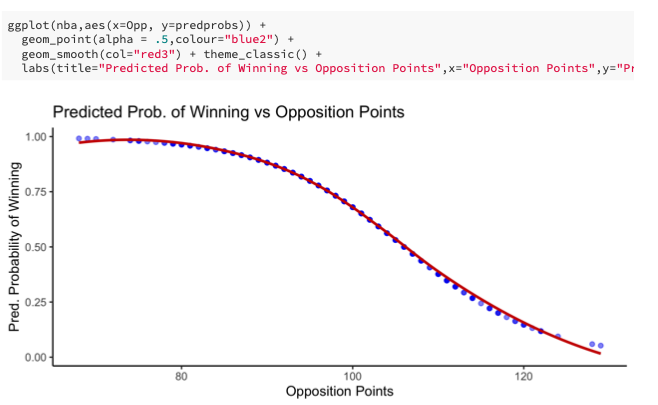
\includegraphics[width=0.5\textwidth]{logit.png} \\
       You learned a \emph{lot}:
       \begin{itemize}
          \item Model selection 
          \item Interpreting BIC, AIC, AUC, R-squared
          \item Residual Plots
       \end{itemize}
       \pause $\Rightarrow$ Develop model to \alert{faithfully represent patterns in the data}
\end{frame}


\begin{frame}[c]{Causal Inference}
  We're focused on what comes \alert{next}.\\
\pause \emph{Assume} our model faithfully represents the data. \\
\pause $\Rightarrow$ \alert{Given those models, what can we conclude \textbf{about the world}?} \\
\vspace*{0.3cm}
\pause Suppose we find a correlation between car advertising and consumer spending across neighborhoods in North Carolina.
\begin{itemize}
  \pause \item Does that imply that more advertising would increase spending further? \\
  \pause In other words, based on this model, do we think advertising is \emph{causing} more consumer spending?
\end{itemize}
\end{frame}

\begin{frame}[c]
  \frametitle{Causal Inference}
\centering
Correlation does not imply causation
\end{frame}

\begin{frame}[c]
  \centering
  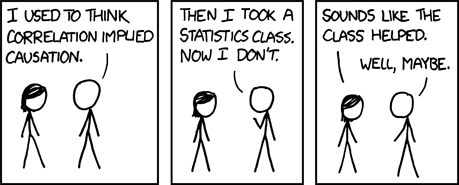
\includegraphics[width=\textwidth]{xkcd_correlation_causation.png}
\end{frame}

\begin{frame}[c]{Causal Inference}
Does advertising cause increased consumer spending?
  \begin{itemize}
  \pause \item ``Well, correlation does not imply causation, so I can't say.''
  \pause \item ``Well, correlation does not imply causation, \emph{but} yea probably.''
\end{itemize}
\end{frame}

\begin{frame}[c]{Causal Inference}
Correlation does not \emph{necessary} imply causation, 
\begin{itemize}
  \pause \item  but when certain assumptions are met, correlation \emph{does} imply causation. 
\end{itemize} 
\vspace*{0.2cm}
\pause By learning the \emph{assumptions} that are required for a correlation to be a good estimate of a causal effect, you can:
\begin{itemize}
  \pause \item Evaluate whether those assumptions are likely to be met,
  \pause \item Come up with different research designs whose assumptions \emph{would} be met. 
\end{itemize}
\end{frame}

\begin{frame}[c]
  \frametitle{Causal Inference}
  \centering
  \textbf{Modeling} \\
  Developing Model to Faithfully Represent Data \\
  \vspace*{1cm}
  $\Downarrow$ \\
  \vspace*{1cm}
   \alert<2->{\textbf{Inference}} \\
  \alert<2->{Interpreting Model Parameters}
\end{frame}

\begin{frame}[c]{Causal Inference}
While we will use a ``statistical framework'' (Potential Outcomes Framework) to help us be rigorous in our thinking... \\
\vspace*{0.2cm}
\pause There are \textbf{NO} statistical tests that will tell you if your model is estimating a true causal effect. \\
\begin{itemize}
  \pause \item \emph{Fundamental Problem of Causal Inference}
\end{itemize}
\vspace*{0.2cm}
\pause Causal inference is \alert{unavoidably} about: 
\begin{itemize}
  \item Critical thinking
  \item Case knowledge
\end{itemize}
\end{frame}

\begin{frame}[c]\frametitle{Causal Inference}
After introducting Potential Outcomes, we'll explore a range of causal research techniques:
\begin{itemize}
  \pause \item Experiments (Randomized-Control Trials, or RCTs)
  \pause \item Linear Regressions as Causal Tools 
  \pause \item Matching 
  \pause \item Differences in Differences
  \pause \item Natural Experiments
\end{itemize}
\pause $\Rightarrow$ Each of these designs will provide causal estimates \alert{if certain assumptions are met}, 
\begin{itemize}
  \pause \item But it will always be is up to you, the researcher, to evaluate whether those assumptions are reasonable!
\end{itemize}
\end{frame}

\begin{frame}[c]{Causal Inference}
  By the end of this course, you will:
  \begin{itemize}
      \item Understand why causal inference is hard, \\
      \pause \item Be able to critically evaluate causal evidence collected by others, \\
      \pause \item Articulate causal questions, \\
      \pause \item And develop research designs to answer those questions. 
  \end{itemize}
  \end{frame}
  
\end{document}
